\documentclass[11pt,a4paper]{DL}
\usepackage[hidelinks]{hyperref}
\usepackage{numprint}
\npthousandsep{,}
\usepackage{multirow} % anforanden
%\usepackage{paralist} % poligraph
\usepackage{listingsutf8} %poligraph
% the package above should be replaced with e.g. the minted library
\usepackage{latexsym} %poligraph
\usepackage{graphicx} %poligraph
\usepackage{longtable}   % tables that can extend over a page
\usepackage[section]{placeins} % to keep floats within sections
\addbibresource{thesis.bib}


\title{Because Democracy}
\subtitle{Computationally Assessing Argumentation in Swedish Parliamentary Debates}

\author{Stian Rødven-Eide}
\pubyear{2025}
\DLno{1337}
\ISBN{123-45-6789-10-11}
\begin{document}

\maketitle
\frontmatter

\begin{abstract}
    Argumentation has been studied since antiquity. Despite its long history and continued prevalence in human communication, computational methods for analysing and assessing argumentation are still limited. The reasons for this are manifold. Argumentation is among the most complex of human interactions, situated in the intersection between logic, rhetoric and pragmatics. This makes it hard even for human annotators to agree on what is argumentation or not. It is also highly domain specific. What is considered an argument in a domestic situation has little bearing in a court. Arguments in social media bear little resemblance to those put forward in parliament.
    
    The task of automatically identifying and classifying argumentation in text is commonly referred to as \emph{argumentation mining}. In contrast to many other NLP tasks, argumentation mining is usually defined as a series of subtasks; no single method can be expected to take you from training data to correctly classified text. Rather, depending on the concrete goal as well as the language domain, a number of interlinked processes are needed, something that makes every argumentation mining project, to a certain degree, unique.
    
    This thesis presents the story of applying argumentation mining techniques to Swedish parliamentary debates. Working on the assumptions that minimising noise in data is particularly crucial, and that the process can be significantly improved by linguistic annotation and additional knowledge, we detail in part two how we created a high quality dataset, augmented with detailed annotation and several knowledge graphs. We demonstrate the issues connected with using standard models for certain classification -- such as named entity recognition and anaphora resolution -- and thus the benefits of fine tuning models on our data.
    
    Part three describes our work on building a specialised argumentation mining pipeline for Swedish parliamentary debates. Here, we go through a number of different approaches, each bringing us a step closer to useful classification of argument components and the relations between them. We will investigate the following hypotheses:
    \begin{itemize}
        \item Due to the formal structure of parliamentary debates, a rule-based method for determining the central claim should work well, while minor claims and premises are better classified using statistical methods.
        \item As a consequence of the complexity of argumentation in this domain, a common pairwise labelling for establishing the argumentative structure will be insufficient. Instead, we a method based on discourse parsing should yield better results.
    \end{itemize}
     
    
    First, however, we introduce the thesis work in more detail in part one, where we explain our reasoning behind this project, as well as a discussion of our challenges, our findings and some ideas for improvement.
\end{abstract}

\begin{sammanfattning}
    Vi är alla sammanfattning.
\end{sammanfattning}

\begin{acknowledgements}
    I would hereby like to thank everyone in the whole wide world.
    
\bigskip

\rightline{Stian Rødven-Eide}

\rightline{Gothenburg, April 19, 2025}
\end{acknowledgements}

\tableofcontents
\mainmatter

\part{Introduction and overview of the thesis work}	%separate page with only title
\label{part:kappa}

\chapter{Introduction}
\label{introduction}
\section{Research questions and contributions}
\label{sec:contrib}

\begin{itemize}
    \item The Swedish parliament regularly debates. These debates are published so and so.
    \item The rather formal language makes NLP easier.
    \item This is where laws and regulations are made.
    \item Because democracy.
    \item As the debates are essentially arguments for or against propositions and motions, argument mining can help us understand:
    \begin{itemize}
        \item how argumentation is done in the parliament (this is vague; a broad perspective),
        \item what types of arguments are used (i.e. schemes),
        \item how arguments are structured (linked, serial, etc),
        \item who generally talks to whom (the macro structure of a debate),
        \item how formalised the debates are (can we infer the debater from a speech?),
    \end{itemize}
    \item and answer research questions such as:
    \begin{itemize}
        \item is there any difference between the different parties' argumentation?
        \item has the type of argumentation changed during the period of my data?
        \item is there any correlation between types of arguments and the votes?
        \item does the debate have any influence on the votes at all?
    \end{itemize}
\end{itemize}

\section{Overview of publications}

The following publications are included in this thesis:

\section{Structure of the thesis}
\label{sec:thesis_struct}

\chapter{Background}
\label{background}
\section{Why we did what we did}
\label{sec:l2-cefr}

Because democracy!

\chapter{Resources}
\label{resources}
In this chapter, we describe the corpora and the lexical resources used to carry out the research and the experiments presented in this thesis.

\chapter{Methods}
\label{methods}
Given the highly interdisciplinary nature of the thesis topic that might attract readers from different disciplines, in this chapter, we introduce the main statistical and machine learning methods underlying the papers listed in parts II and III. Clarification on some additional methods employed are detailed in the relevant publications.

\chapter{Discussion}
\label{discussion}
In this chapter, we provide an overview of the main findings and contributions arising from this thesis work.

\chapter{Conclusion}
\label{conclusion}
\section{Summary}
%Summarize findings but also compare the research questions and conclusions 

It all comes together!

\section{Future directions}

Much to do!

\section{Significance}

Very important!

\part{From text to propositions}

\chapter{The politicians}
\label{poligraph_paper}
\UseRawInputEncoding

\textbf{Abstract.} As part of a larger project on argument mining of Swedish parliamentary data, we have created a semantic graph that, together with named entity recognition and resolution (NER), should make it easier to establish connections between arguments in a given debate. The graph is essentially a semantic database that keeps track of Members of Parliament (MPs), in particular their presence in the parliament and activity in debates, but also party affiliation and participation in commissions. The hope is that the Swedish PoliGraph will enable us to perform named entity resolution on debates in the Swedish parliament with a high accuracy, with the aim of determining to whom an argument is directed.

\section{Introduction}

While argument mining still is a young task in the field of computational linguistics, it has received much attention during the last five years. Parliamentary data is not only an ideal application of this, but also often a treasure trove of training data, given its standardised language and detailed accompanying metadata. Debates from the Swedish parliament, which will be the main focus for this project, are available from 1971 until the present date, with particularly detailed metadata present from 1993 and onward. The ultimate task of our project is to evaluate and develop tools for argument mining on these debates. As a first step, we have created the Swedish PoliGraph, a semantic graph to aid us in achieving our goal. Following the completion of this graph, we will use it to improve upon methods for NER that, in turn, can assist in determining the structure of discourse present in the various debates in the Swedish parliament.

\section{About the Swedish Parliamentary Data}

Coinciding with the ratification of \emph{Lag (2010:566) om vidareutnyttjande av handlingar från den offentliga förvaltningen}, a law commonly known as \emph{PSI-lagen} `re-use of Public Sector Information', \emph{Riksdagens öppna data} `parliamentary open data', from here on abbreviated as RÖD) was published in 2010. A massive collection of structured content from the databases of the Swedish parliament, RÖD is continuously updated, both with new data and with the gaps in older data filled in.

The available data is sorted into five categories: Documents, MPs, voting results, speeches and calendar. Of these, the documents constitute the largest category, with a substantial amount of data from 1971 and onward. The categories for MPs and voting results consist mostly of metadata, while speeches are transcripts of both addresses and replies, accompanied by extensive metadata, starting from 1993.\footnote{An exhaustive description of the various available datasets cannot be given in this paper. The documents category in particular contains 40 different types of documents. Please see the RÖD website at \url{https://data.riksdagen.se/} and Riksdagen's page for descriptions of the various document types at \url{https://www.riksdagen.se/sv/Dokument-Lagar/}.}

In addition to their availability through a well documented API, the data can be downloaded in several formats, including HTML, plain text, CSV, XML, JSON and SQL.

For the initial stages of this project, we choose to focus on the speeches category (\emph{anföranden} in Swedish), as this dataset is relatively consistent, fairly complete and contains the most metadata. Once we have developed our methods for argument mining, we can extend the data to include older protocols from debates dating back to 1971. A \emph{speech} in this context refers to an entry in a debate, and the term will be used in this sense throughout the paper.

\section{Development Details}

\subsection{The RÖD Documents}

After removing a small number of ill-formed documents, we ended up with 325\,202 speeches in our dataset. Starting with the downloads from RÖD in JSON format, each speech is one document, and constitutes one entry in a debate in the Swedish parliament. Most debates are on specific propositions from either the government, parliamentarians or commissions, though there are also weekly meetings in the parliament where MPs can address ministers directly with questions. Debates usually end with a voting session, the details of which are stored in a different dataset. At a later stage, we will combine our argument analysis with the votes in order to better understand the relationship between debates and the resulting votes.

\subsection{Speeches}

A typical speech document contains the metadata as outlined in table \ref{poli-anf-table}. Of particular importance here is \emph{dok\_id}, which designates the meeting in question, \emph{anforande\_nummer}, referring to the number of this speech in the chronological order of speeches during that meeting, and \emph{rel\_dok\_id}, which is the ID of the proposition that is being debated. In order to map a single debate, we therefore need to:

\begin{enumerate}
    \item Find all speeches with a given \emph{rel\_dok\_id}.
    \item Determine the meeting(s) this was debated in.
    \item Establish the chronological order of the speeches during these meetings.
    \item Analyse each speech and attempt to determine which previous speech or speeches (if any) was/were addressed or argued against.
\end{enumerate}

\subsection{Members of Parliament}
\label{sec:mp}

For the Swedish PoliGraph, we have combined the speech information with metadata from the MP category, which includes basic biographical information as well as a complete history of their roles in the parliament. Such roles are usually their time working as an MP and commission work, but also longer sick leave is listed here as well as their substitutes in those cases. In addition to the essential identifiers ``name'' and ``party'', mappings are also created to MP's Wikidata-IDs and their listed name there, which sometimes provide more detail than the names as they are stored in RÖD.

The roles of MPs are generally described in terms of positions, where each assignment (or leave from that assignment) is stored as a factual predicate with eight arguments:
\begin{enumerate}
    \item MP-ID\\ \emph{A unique ID for each MP.}
    \item Agency code\\ \emph{An identifying code for the agency. This can be ambiguous, as parties and commissions sometimes use the same identifier.}
    \item Role\\ \emph{The MP's role in the agency, e.g. parliamentarian, commission chair or substitute.}
    \item From\\ \emph{Starting date of the position.}
    \item To\\ \emph{End date of the position.}
    \item Type\\ \emph{The type of position, usually either ``kammaruppdrag'' for the parliament or ``uppdrag'' for commission work.}
    \item Uppdrag\\ \emph{The info here varies. For commission work and other extraparliamentary duties, it contains the full name of the commission or equivalent. For extended leave, it lists the name of substitutes.}
    \item Status\\ \emph{The MP's presence or absence during the given period.}
\end{enumerate}

\begin{table}[t!]
\begin{center}
\begin{tabular}{|l|l|}
\hline \textbf{Property} & \textbf{Description} \\ \hline
dok\_hangar\_id & Internal document ID \\
dok\_id  & Meeting + speech no. \\
dok\_titel & Protocol title \\
dok\_rm & Parliamentary year \\
dok\_nummer & Number of meeting \\
dok\_datum & Date of speech \\
avsnittsrubrik & Topic title \\
underrubrik & Topic subtitle \\
kammaraktivitet & Type of debate \\
anforande\_id & Unique speech ID \\
anforande\_nummer & Speech number in debate \\
talare & Speaker name \\
parti & Speaker party \\
anforandetext & Full speech text \\
intressent\_id & Speaker's ID \\
rel\_dok\_id & Document being debated \\
replik & Speech type \\
systemdatum & Date of publishing \\
\hline
\end{tabular}
\end{center}
\caption{\label{poli-anf-table} A typical speech document. }
\end{table}

\begin{figure*}
 \centering 
 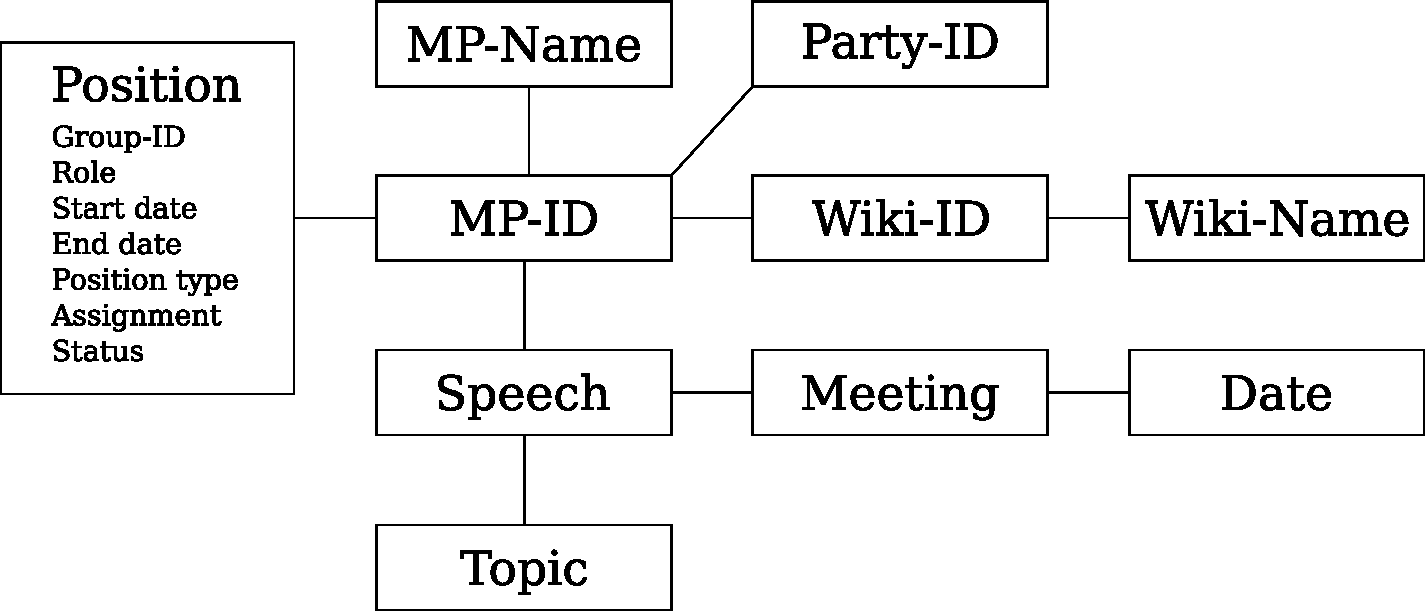
\includegraphics[width=12cm]{images/graph-drawing.pdf}
 \caption{\label{mp-graph} A semantic graph of Swedish MPs and debates.}
\end{figure*}

\subsection{Implementation}

For our rendering of these data as a semantic graph, we chose to create a deductive database in SWI-Prolog, and combine it with the Pengines framework in order to offer web access. Prolog's modular nature allows for very quick prototyping and makes it easy to combine existing rules instead of writing complicated queries such as would be required with SQL or SPARQL. With Pengines, web access is offered simultaneously through a web interface and RPC (Remote Procedure Call) commands passed directly to the server from any Prolog client \cite{lager_pengines_2014}.



Our Prolog database ended up consisting of a number of files, each mapping identifiers and properties to each other. In order to make NER as accurate as possible, we created mappings to MPs' names both as they are listed in the Swedish parliament and how they appear on Wikipedia. This, of course, includes a mapping between unique MP IDs in the parliament and their respective Wikidata-ID, which can potentially be of use for further integration with other analytical tools. For MPs, we also created a file listing their party affiliation that probably will be a necessary step in resolving name ambiguity, as well the previously mentioned position file that details their formal time in parliament and and activity in various commissions. Finally, we have two files that map meetings to dates and debate topics, respectively. An approximation of the resulting graph can be seen in figure \ref{mp-graph}.\footnote{An approximation in the sense that Prolog predicates can have any number of arguments. The Speech and Meeting nodes are for instance mapped to MP-ID and each other in the same predicate.} The edges should be read as \emph{has} or \emph{is}, with either MP-ID or the node closest to it as the subject.

\section{Usage Details}

The Swedish PoliGraph is available to use and download from \url{https://spraakbanken.gu.se/poligraph/} under a Creative Commons Attribution licence.\footnote{\url{https://creativecommons.org/licenses/by/4.0/}} We ask that this paper be cited in any published work using the code or the graph.

\subsection{Rule Construction}

In contrast to relational database queries, Prolog queries are largely dependent on rule construction. For the Swedish PoliGraph, we have created a small set of specialised rules for the purpose of disambiguating names and titles that specifically refer to MPs. A Prolog rule is essentially a list of predicates that must be true in order to satisfy a query. These predicates can be either facts or other rules. Any argument can be substituted with a variable that will, when queried, provide any answer for which that predicate would be true. To give an example, a rule stating that a given politician was an elected and working MP on a given date would be:

\begin{lstlisting}
was_in_rd(Name, Date) :-
    rid_sname(Rid, Name),
    position(Rid,'kam',_,From,Tom,_,_,Status),
    Date >= From,
    Date =< Tom,
    Status \= 'Ledig'.
\end{lstlisting}
%
In somewhat clearer English, this rule states that: A person with a given \emph{Name} was an elected and working MP on a given \emph{Date} \textbf{IF} there exists a mapping from that name to an MP-ID \textbf{AND} that MP-ID had a position in \emph{kam} (eng: the parliament) in that period \textbf{AND} their status in that time was not \emph{Ledig} (eng: away).

\subsection{Using the Swedish PoliGraph}

There are three ways of using the Swedish PoliGraph: (1) local querying with SWI-Prolog; (2) remote querying with SWI-Prolog and Pengines; and (3) via the web interface. Of these, the latter will necessarily be more limited in functionality than the other two, since a practically usable web interface will not be able to reproduce the flexibility that Prolog queries provide.

\begin{table*}[t!]
\fontsize{10pt}{12pt}\selectfont
\begin{center}
\begin{tabular}{|l|l|}
\hline \textbf{Predicate} & \textbf{Description} \\ \hline
\texttt{rid\_sname/2} & Maps an MP-ID to that person's sorting name, e.g. 'Löfven,Stefan' \\
\texttt{rid\_wname/2} & Maps an MP-ID to that person's Wikipedia name, e.g. 'Stefan Löfven' \\
\texttt{rid\_lname/2} & Maps an MP-ID to that person's last name \\
\texttt{rid\_fname/2} & Maps an MP-ID to that person's first name \\
\texttt{rid\_name/2} & Maps an MP-ID to any of the names above \\
\texttt{rid\_wid/2} & Maps an MP-ID to that person's Wikidata-ID \\
\texttt{rid\_party/2} & Maps an MP-ID to that person's party affiliation \\
\texttt{position/8} & See section \ref{sec:mp} for details \\
\texttt{anforande/3} & Maps a speech to a meeting number (dok\_id) and an MP-ID \\
\texttt{dokid\_date/2} & Maps a meeting number (dok\_id) to its date \\
\texttt{meet\_anf\_topic/3} & Maps a topic to a meeting number (dok\_id) and a speech number \\
\texttt{had\_previous\_anf/8} & Matches previous speeches. See section \ref{sec:querying} for details\\
\texttt{had\_anf/6} & Gives speeches with topic, speaker, speech number, 
   party and dok\_id  \\
\texttt{had\_anf/4} & Gives the name, ID and party affiliation for all speeches
   on a given date \\
\texttt{was\_in\_rd/3} & Who was in the parliament in a given period \\
\texttt{was\_mp/3} & Who was an elected MP (non-minister) in a given period \\
\texttt{was\_minister/3} & Who was a minister in a given period \\
\texttt{was\_ledig/3} & Who was on leave from the parliament in a given period \\
\texttt{has\_position/3} & A simplification of position/8 --
   Matches MP's to their assignments \\
\hline
\end{tabular}
\end{center}
\normalfont
\caption{\label{pred-table} A list of currently defined predicates. }
\end{table*}

\subsubsection{Local Querying}
\label{sec:querying}

A central feature of Prolog as a programming language is its \emph{declarative} nature. A Prolog program consists of facts and rules, and are usually interacted with in terms of queries, not unlike relational databases. For the Swedish PoliGraph, we have defined a number of predicates that can be queried directly, although it is also possible for a user to define new predicates extending or combining the existent ones.

In order to start using the Swedish PoliGraph locally, start SWI-Prolog and load the main program file with \texttt{[poligraph].} There you will be able to query both the basic facts and the more complex rules. Note that for any argument, you can use either a quoted string or a number to search for an exact match, or use an upper-case string for a variable. Some simple examples are as follows:

\begin{lstlisting}
/* ID of any MP with last name 'Löfven' */
?- rid_lname(Rid,'Löfven').
Rid = 218878014918.

/*Wikidata-ID for an MP-ID */
?- rid_wid(218878014918, Wid).
Wid = 'Q2740012'.

/* Party affiliation for an MP-ID */
?- rid_parti(218878014918, Party).
Party = 'S'.
\end{lstlisting}
%
%Note here that we have used the term \emph{Rid} to signify an MP's unique ID in the Swedish Parliament, otherwise refered to as MP-ID in this paper.
%, and that we have separate predicates for mapping the MP-ID to last name (\texttt{rid\_lname/2}), first name (\texttt{rid\_fname/2}), sorting name (\texttt{rid\_sname/2}) and Wikidata-name (\texttt{rid\_wname/2}), though they can all be queried simultaneously with \texttt{rid\_name/2}.
The main predicate, however, is constructed for the following purpose: We have a speech, in which a name is mentioned. In order to resolve the name, we wish to see who by that name was talking previously in the same debate. Preferably we know both the meeting number (\emph{dok\_id}) and the topic (\emph{rel\_dok\_id}). As an example, in a debate on 2016-12-12 on the topic of communication infrastructure, MP Teres Lindberg mentioned an Erik Ottoson in her speech, which was the 75th speech in that debate. Querying our program, we get the MP-ID, party affiliation and speech number(s) for that person's earlier participation in the debate: %Kanske du vill skriva att om det bara stått Ottoson så kunde vi fått en lista med alla Ottoson som tidigare pratat i debatten och därmet gjort lite disambiguering direkt? På det viset blir det ännu tydligare vad styrkan och värdet med Poligraph är!


\begin{lstlisting}
?- had_previous_anf('Erik Ottoson', Rid, Anf, Party, 'H401TU1', 'H40944', 75, _).
Rid = 832311880029,
Anf = 74,
Party = 'M' ;
Rid = 832311880029,
Anf = 72,
Party = 'M' ;
\end{lstlisting}
%
In more complex cases, a speaker may not provide the full name of the person they refer to, but rather just their last name or a phrase that only includes their party affiliation. We can then use the same predicate, retrieving the same information plus any additional matches. Where there exists ambiguity in the results, such as several people with the same last name or party affiliation, we can apply simple heuristics, e.g. the last speech before the current speaker's, to identify our target.

In a given query, any of the information we provide can be substituted with a variable, or vice versa. This means that we can get all speeches from a given party in a given debate by using variables for everything except Party and Topic:

\begin{lstlisting}
?- had_anf(Name, Rid, Anf, 'S', 'H401TU1', Meeting).
Name = 'Lindberg',
Rid = 559925283228,
Anf = 73,
Meeting = 'H40944' ;
Name = 'Johansson',
Rid = 691264514114,
Anf = 63,
Meeting = 'H40944' ;
\end{lstlisting}
%
A complete list of currently defined predicates can be seen in table \ref{pred-table}. 

\subsubsection{Remote Querying with Pengines}

By using the Pengines library for SWI-Prolog, the Swedish PoliGraph can be queried remotely. This works essentially the same as local querying, except that the query is wrapped in a predicate \texttt{pengine\_rpc/3}.\footnote{The trailing \texttt{/3} is a Prolog convention to show the arity of a predicate.} The predicate takes three arguments: The URL of the Pengines server, the predicate you wish to run and a list of options, which must include the name of the application on the server. Submitting our previous example over \texttt{pengine\_rpc/3} would look like this:

\begin{lstlisting}
?- pengine_rpc(
  'https://spraakbanken.gu.se/poligraph/',
  rid_lname(Rid,'Löfven'),
  [application(poligraph)]
).
\end{lstlisting}
%
Pengines also allows for several other options, such as specifying which information should be transferred between the client and the server and passing user-created predicates to be used in the query. For details on these options, we refer to Lager and Wielemaker \cite{lager_pengines_2014} and the official Pengines documentation\footnote{\url{http://www.swi-prolog.org/pldoc/package/pengines.html}}.



\subsubsection{The Web Interface}

The web interface is by necessity simplified and only allows for a few selected queries. As such it is primarily intended for demonstration purposes, but it can also be used for qualitative research.



\section{Related Work}

While argumentation mining is a recent field of study where little has been done on parliamentary data (see e.g. \cite{lippi_argumentation_2016} for a good overview), semantic networks are almost as old as computers themselves, starting with a linguistic application by the Cambridge Language Research Unit in 1956 \cite{lehmann_semantic_1992}. An essential part of the semantic web, there now exist large-scale semantic graphs on most subjects, the most comprehensive project being the Wikipedia-sourced DBpedia \cite{lehmann_dbpedia_2015}. For parliamentary data, the situation has improved over the last few years, and with the increasing implementation of public open data policies we can expect to see much further work in that domain. To our knowledge, the largest project for creating a semantic network from parliamentary data was Talk of Europe, which resulted in the LinkedEP Dataset \cite{hollink_talk_2017}, covering all plenary debates held in the European Parliament between July 1999 and July 2017 \cite{van_aggelen_debates_2017}, as well as biographical information about the members of parliament sourced from Høyland et al. \cite{hoyland_forum_2009}. We have also seen this inspire national efforts such as Talk of Norway \cite{lapponi_talk_2018}, while several earlier projects are mentioned by Van Aggelen et al. \cite{van_aggelen_debates_2017}.

\section{Conclusions and Future Work}

We have created the Swedish PoliGraph specifically for named entity resolution and argumentation mining, and hope that it will prove fruitful to that end. Our next step will be NER, and while the current version of the graph is tailored for this, future needs may encourage us to augment it with further metadata, e.g. as additional features to be used in argumentation mining.

We also hope that this graph can be useful outside of our planned scope. The Swedish PoliGraph is both detailed and flexible enough that it can purposefully serve any project dealing with Swedish MPs and debates, be it academic, educational or journalistic.

\chapter{The debates}
\label{anforanden_paper}
\UseRawInputEncoding


\textbf{Abstract.} The Swedish parliamentary debates have been available since 2010 through the parliament's open data web site \emph{Riksdagens öppna data}. While fairly comprehensive, the structure of the data can be hard to understand and its content is somewhat noisy for use as a quality language resource. In order to make it easier to use and process -- in particular for language technology research, but also for political science and other fields with an interest in parliamentary data -- we have published a large selection of the debates in a cleaned and structured format, annotated with linguistic information and augmented with semantic links. Especially prevalent in the parliament's data were end-line hyphenations -- something that tokenisers generally are not equipped for -- and a lot of the effort went into resolving these. In this paper, we provide detailed descriptions of the structure and contents of the resource, and explain how it differs from the parliament's own version.


\section{Introduction}

Since the freedom of information acts started becoming implemented in various countries, we have seen a plethora of parliamentary corpora being released and enhanced, by governments as well as researchers. Significant corpora have been published e.g. from the parliaments of Norway \cite{lapponi_talk_2018}, Slovenia \cite{pancur_slovparl_2018} and the UK \cite{nanni_ukparl_2018}, to name but a few.

This paper presents and describes a corpus of Swedish parliamentary debates that has been adapted from the parliament's data. In order to make it easier for further research on this data -- the government's own version has also been somewhat underdocumented -- we have devoted section \ref{contents-structure} to a detailed description of the content and structure of the corpus and the accompanying metadata. In section \ref{processing-corpus} we present our improvements to the resource, in particular the handling of prevalent end-line hyphenations.

The word \emph{anförande} (plural: \emph{anföranden}) refers to any entry in the Swedish parliamentary debates. While the most reasonable translation into English is \emph{speech}, an \emph{anförande} in this context can also be a short reply to a previous speech. For the remainder of this article, however, we will use the term \emph{speech} for all debate entries, and \emph{anföranden} only when referring to the resource as a whole.

\begin{center}
\begin{longtable}{|l|r|}
\hline
\normalsize{\textbf{Type}} & \normalsize{\textbf{Amount}} \\ \hline
None & 139,446 \\ \hline
interpellationsdebatt & \multirow{2}{*}{61,781} \\ \emph{interpellation debate} & \multicolumn{1}{c|}{} \\ \hline
föredragning av utskottsärende & \multirow{2}{*}{58,381} \\ \emph{presentation of committee report} & \multicolumn{1}{c|}{} \\ \hline
frågestund & \multirow{2}{*}{20,975} \\ \emph{question time} & \multicolumn{1}{c|}{} \\ \hline
ärendedebatt & \multirow{2}{*}{16,947} \\ \emph{legislative debate} & \multicolumn{1}{c|}{} \\ \hline
allmänpolitisk debatt & \multirow{2}{*}{7,906} \\ \emph{general policy debate} & \multicolumn{1}{c|}{} \\ \hline
partiledardebatt & \multirow{2}{*}{3,616} \\ \emph{party leader debate} & \multicolumn{1}{c|}{} \\ \hline
frågestund med statsministern & \multirow{2}{*}{2,878} \\ \emph{Prime Minister's question time} & \multicolumn{1}{c|}{} \\ \hline
aktuell debatt & \multirow{2}{*}{2,601} \\ \emph{topcial debate} & \multicolumn{1}{c|}{} \\ \hline
information från regeringen & \multirow{2}{*}{2,411} \\ \emph{information from the government} & \multicolumn{1}{c|}{} \\ \hline
bordläggning & \multirow{2}{*}{1,441} \\ \emph{tabling} & \multicolumn{1}{c|}{} \\ \hline
val & \multirow{2}{*}{1,306} \\ \emph{election} & \multicolumn{1}{c|}{} \\ \hline
utrikespolitisk debatt & \multirow{2}{*}{1,241} \\ \emph{foreign policy debate} & \multicolumn{1}{c|}{} \\ \hline
statsministerns frågestund & \multirow{2}{*}{1,098} \\ \emph{Prime Minister's question time} & \multicolumn{1}{c|}{} \\ \hline
debatt vid allmän debattimme & \multirow{2}{*}{858} \\ \emph{hour of general debate} & \multicolumn{1}{c|}{} \\ \hline
särskild debatt & \multirow{2}{*}{536} \\ \emph{special debate} & \multicolumn{1}{c|}{} \\ \hline
avgörande av utskottsärende & \multirow{2}{*}{512} \\ \emph{decision on committee proposal} & \multicolumn{1}{c|}{} \\ \hline
budgetdebatt & \multirow{2}{*}{401} \\ \emph{budgetary debate} & \multicolumn{1}{c|}{} \\ \hline
meddelande & \multirow{2}{*}{323} \\ \emph{message} & \multicolumn{1}{c|}{} \\ \hline
hänvisning till utskott & \multirow{2}{*}{236} \\ \emph{referral to committee} & \multicolumn{1}{c|}{} \\ \hline
avlämnande av regeringsförklaring & \multirow{2}{*}{72} \\ \emph{submission of government declaration} & \multicolumn{1}{c|}{} \\ \hline
återupptagning av förhandlingarna & \multirow{2}{*}{67} \\ \emph{resumption of negotiations} & \multicolumn{1}{c|}{} \\ \hline
ceremoni & \multirow{2}{*}{47} \\ \emph{ceremony} & \multicolumn{1}{c|}{} \\ \hline
beslutsfattande om uppdrag & \multirow{2}{*}{46} \\ \emph{assignment decision} & \multicolumn{1}{c|}{} \\ \hline
återrapportering & \multirow{2}{*}{36} \\ \emph{report} & \multicolumn{1}{c|}{} \\ \hline
anmälan & \multirow{2}{*}{31} \\ \emph{notification} & \multicolumn{1}{c|}{} \\ \hline
riksmötets öppnande & \multirow{2}{*}{6} \\ \emph{parliamentary opening} & \multicolumn{1}{c|}{} \\ \hline
regeringsförklaring & \multirow{2}{*}{2} \\ \emph{declaration of government} & \multicolumn{1}{c|}{} \\ \hline
hälsningsanförande & \multirow{2}{*}{1} \\ \emph{welcoming speech} & \multicolumn{1}{c|}{} \\
\hline
\caption{\label{kam-table} Types of parliamentary activity.  }
\bigskip
\end{longtable}
\end{center}

\section{\label{contents-structure}Content and structure of the corpus}

The Swedish parliament has published minutes for all parliamentary debates from 1971 and onward.\footnote{\url{http://data.riksdagen.se/data/dokument/}} These files are derived from scans of printed or typed documents and the large amount of HTML formatting present in the files are only for preserving layout; it does not generally segment the text in a way that helps with parsing. Metadata is restricted to document level information, and as such does not say anything about which speakers participate or which topics are being discussed.

However, all debates from 1993 and onward are also available in a separate dataset aptly named \emph{anföranden}, where each speech is complemented with appropriate metadata such as speaker, party, topic and speech order.\footnote{\url{http://data.riksdagen.se/data/anforanden/}} This is the resource that we have enhanced.

\subsection{\label{resource-contents}Resource size and contents}

After removing 20 empty documents from the parliament's data, we have \numprint{325202} speeches, the speech texts of our cleaned version containing \numprint{122079937} tokens as measured with the Spacy tokeniser.\footnote{\url{https://spacy.io/}} This gives an average of 375.4 tokens per speech.

To get a better sense of the contents of the resource, we refer to table \ref{kam-table}. The property \emph{kammaraktivitet} (chamber activity) in each document provides an indication to the context of the text. Unfortunately, this is not applied entirely consistently across all documents. For instance, questions to the prime minister can be found under both \emph{statsministerns frågestund} and \emph{frågestund med statsministern}. More importantly, however, most of the regular debates have no value for this property; they are in the table listed as \emph{None}. On the other hand, some of them do have a label; most of the categories whose descriptions contain the word \emph{debatt} are the types of regular debates that also dominate the category \emph{None}. For any research pertaining strictly to the debates, our recommendation is therefore to exclude the categories we know are not debates rather than vice versa. % Maybe you should keep all recommendations in one paragraph at the end? if there are more recommendations, if not, just keep it as it is. 



\subsection{Document structure}

In table \ref{anf-table}, we show the complete structure of a typical speech document. In our version of the corpus, all properties except for \emph{anförandetext} (speech text) are XML attributes of the speech as a whole. These attributes have been transferred directly from the parliament's data, with the exception of \emph{dok\_datum} which erroneously listed all parliamentary sessions as having taken place at midnight; for this reason, we removed the time stamp from the data, leaving only the dates, which are correct.

\begin{table}[ht!]
\begin{center}
\begin{tabular}{|l|l|}
\hline \textbf{Property} & \textbf{Description} \\ \hline
dok\_hangar\_id & Internal document ID \\
dok\_id  & Meeting + speech no. \\
dok\_titel & Protocol title \\
dok\_rm & Parliamentary year \\
dok\_nummer & Number of meeting \\
dok\_datum & Date of speech \\
avsnittsrubrik & Topic title \\
%underrubrik & Topic subtitle \\
kammaraktivitet & Type of debate \\
anforande\_id & Unique speech ID \\
anforande\_nummer & Speech number in debate \\
talare & Speaker name \\
parti & Speaker party \\
anforandetext & Full speech text \\
intressent\_id & Speaker's ID \\
rel\_dok\_id & Document being debated \\
replik & Speech type \\
systemdatum & Date of publishing \\
\hline
\end{tabular}
\end{center}
\caption{\label{anf-table} A typical speech document. }
\end{table}

\begin{itemize}
    \item \textbf{dok\_hangar\_id} is a unique and strictly numerical ID which is assigned to every document in the parliament's database. It is not referenced in other documents, however, and can normally be safely ignored.
    \item \textbf{dok\_id} is a unique ID (different from dok\_hangar\_id) assigned to every document in the parliament's database. In contrast to the above, dok\_id is alphanumeric and referenced by other documents. Its form is derived from a set of codes that signify the time and type of the document. The two first characters refer to the parliamentary period in which the document was created, the third and fourth characters refer to the type category to which the document belongs, while the remaining characters signify a category subtype and/or number within its category. In this dataset, the category is consistently 09, meaning \emph{minutes from the chamber}, with the subsequent digits representing the chronological number of the meeting within the parliamentary year, corresponding to dok\_nummer below.
    A more detailed description of the dok\_id format is available on the Swedish parliament website.\footnote{\url{http://data.riksdagen.se/dokumentation/sa-funkar-dokument-id/}}
    \item \textbf{dok\_titel} is a human readable label that for this dataset consistently states that it is the minutes from a given parliamentary session. While it does contain an hour / minute time reference, this refers to the time of the session and not of individual speeches during the session.
    \item \textbf{dok\_rm} refers to the parliamentary period. Since the autumn of 1975, a parliamentary period lasts from the beginning of an autumn until the end of spring the following year. The format used here is e.g. 2015/16.
    \item \textbf{dok\_nummer} is the chronological number of the parliamentary session within a parliamentary year. %The number of sessions in a year usually range between 120 and 130.
    \item \textbf{dok\_datum} refers to the date of the parliamentary session, using the format YYYY-MM-DD.
    \item \textbf{avsnittsrubrik} is a text label that for debates generally is informative, describing what is being debated. During a parliamentary session, it is common that several topics are debated, each usually from the premise of a proposal pertaining to legal or budgetary matters. The exact proposal being discussed is referenced by rel\_dok\_id below, while this label ranges from general topics such as `climate politics' to rather specific ones such as `increased possibilities of travelling within the European Union using national identity cards'. Not all categories of parliamentary activity feature an informative label, however; e.g. question time or debates between party leaders are only labelled with their respective categories as listed in table \ref{kam-table}.
    \item \textbf{kammaraktivitet} refers to the type of parliamentary activity, as we described above in section \ref{resource-contents} and listed in table \ref{kam-table}.
    \item \textbf{anforande\_id} is another unique alphanumeric ID assigned to each speech. As with dok\_hangar\_id, this is currently not referenced by other documents in the parliamentary database.
    \item \textbf{talare} is a string containing the name and party affiliation of the current speaker. For acting ministers, their title is usually also included, e.g. `Finansministern Magdalena Andersson (S)'
    \item \textbf{parti} is a string containing only the party affiliation of the current speaker. This is listed using the common abbreviations for Swedish political parties, all currently with one or two letters.
    \item \textbf{anforandetext} is the transcribed speech.
    \item \textbf{intressent\_id} is a unique ID number for the speaker. Each member of parliament since 1990 (as well as some before that) is assigned an ID of this type. This can be used to cross-reference with other data sources, as we will demonstrate later.
    \item \textbf{rel\_dok\_id} is a reference to the dok\_id of whatever document is being discussed. Usually, what is being debated is some kind of proposal, from the parliament, the government, or from a commission. The formal document detailing this proposal features the dok\_id referenced here. As such, it can be cross-referenced with a database containing proposals. Also, for many purposes of linguistic mining or classification, it can be more reliable as a topic than the avsnittsrubrik mentioned above.
    \item \textbf{replik} is a binary string, `Y' if the speech is of the type \emph{replik} (reply), `N' if not. While many of the speeches not marked as \emph{replik} may also contain or be regarded as replies to previous speeches, a \emph{replik} is subject to slightly different rules than other speeches, the most significant being that they are much shorter.
    \item \textbf{systemdatum} refers to the date and time when the document was published to the parliament's database.
\end{itemize}

\section{\label{processing-corpus}Processing the corpus}

In this section, we detail our effort to improve the resource.

\subsection{Cleaning}

Although the digitisation of the Swedish parliamentary debates has involved optical character recognition (OCR) as part of the process, our relatively thorough manual investigation found that the result is, for the most part, excellent. There are very few typos or other indications of OCR errors. However, one particularly visible result of this process is the abundant prevalence of end-line hyphenations.

Generally, end-line hyphenation has been ignored by tokenisers, as they do not know whether to join the tokens together as a single word, join them as a hyphenated compound, or leave it as a hanging hyphen (used in elliptical constructions of a conjunction of several terms) \cite{grefenstette_what_1994,frunza_trainable_2008}.

The commonly used tokenisers, most notably the widely used Stanford tokeniser, ignore this problem \cite{manning_stanford_2014}, and while projects such as \cite{dridan_tokenization_2012} and \cite{graen_cutter_2018} suggest useful improvements in the area, the focus is on multi-lingual approaches which would have a hard time capturing the variety of Swedish compounds.

Due to Swedish compounding rules, where basically any number of nouns can be joined together, a pure dictionary approach is insufficient, and parliamentary debates in particular do contain a lot of hanging hyphens. This means that from the outset, a rule based approach to fixing end-line hyphenation needs to account for language specific features and preferably be complemented by manual corrections in order to reach a high accuracy.

One solution is of course to ignore them and treat them as noise, which often makes sense for large corpora where the amount of end-line hyphenation is negligible. For our anföranden, however, we found that not only were they especially prevalent, but that it often is longer low-frequency words that have been split. Such words can make a significant difference in several methods for information retrieval, text mining, and user modelling, which often use term frequency–inverse document frequency (tf-idf) or similar term weighting systems \cite{beel_research-paper_2016}.

We therefore devised a rule-based method, which combined corpus look-up with hand-crafted rules and an interactive query allowing for simple manual correction of those cases that could not be resolved automatically. The procedure was as follows:

\begin{table}[t!]
\begin{center}
\begin{tabular}{|l|l|r|}
\hline \textbf{Conjunction} & \textbf{English} & \textbf{Amount} \\ \hline
och & and & 90,025 \\
eller & or & 3,225 \\
som & as & 1,848 \\
men & but & 1,379 \\
samt & and & 744 \\
till & to & 186 \\
respektive & respectively & 172 \\
än & yet & 35 \\
utan & without & 6 \\
såväl & as well as & 7 \\
og & and (Norwegian) & 4 \\
und & and (German) & 4 \\
kontra & versus & 3 \\
framför & before & 2 \\
liksom & as & 2 \\
snart & soon & 1 \\
inklusive & inclusive & 1 \\
o & and (shortened) & 1 \\
\hline
SUM & & 97,645 \\
\hline
\end{tabular}
\end{center}
\caption{\label{konj-table} Conjunctions in elliptical componds. }
\end{table}


\begin{enumerate}
    \item Generate a word frequency list from the resource. This will be used to decide whether line-end hyphenations should be kept or joined, with or without a hyphen.
    \item Remove all line breaks. The reason for doing this instead of keeping the line break as a signifying feature is that there were several cases of end-line hyphenation in-line, indicating either OCR errors or several layers of OCR processing having been done.
    \item Filter out all cases where the word after the hyphen is a conjunction. These cases are almost certainly part of an elliptical construction and should be kept as is. An overview of the frequency of the different conjunctions in elliptical compounds of several terms in the resource can be found in table \ref{konj-table}.
    \item Use regular expression matching to identify structures that almost certainly should be hyphenated compounds. These are:
    \begin{enumerate}
        \item All characters before the hyphen are upper-case and all characters after the hyphen are lower-case. This indicates an acronym used as a semantic qualifier.
        \item The words before and after the hyphen are both capitalised. This indicates a proper name, which for some people and organisations is hyphenated in Swedish.
        \item All characters before the hyphen are numerals, while the characters after the hyphen are not. This is common in Swedish, e.g. for time references such as \emph{1990-talet}, `the 1990s'.
        \item The word \emph{icke}, `not', is particular to Swedish for requiring a hyphen when used as a prefix.
    \end{enumerate}
    An overview of these can be seen in table \ref{regex-table}.
    \item Generate two word forms comprising all characters before and after the hyphen, one joined with hyphen and one joined without. Check whether any or both of these are present in the word frequency list. If only one is present, choose that. If both are present, choose the one that is most frequent. If both are either missing or equally frequent, ask the user what to do.
    \item Whenever a selection has been made, either by the heuristics or the user, save that selection and apply it to subsequent identical cases.
\end{enumerate}

\begin{table}[t!]
\begin{center}
\begin{tabular}{|l|r|r|}
\hline \textbf{Regular expression} & \textbf{Unique} & \textbf{Total} \\ \hline
(a) {[A-ZÅÄÖ]}+- [a-zåäö]+ & 2,527 & 7,740 \\
(b) {[A-ZÅÄÖ][a-zåäö]+-} & & \\
\hspace{1.4em}{[A-ZÅÄÖ][a-zåäö]+} & 338 & 1,560 \\
(c) \textbackslash d+- \textbackslash w+ & 949 & 2,802 \\
(d) icke- \textbackslash w+ & 162 & 283 \\
\hline
SUM & 3,976 & 12,385 \\
\hline
\end{tabular}
\end{center}
\caption{\label{regex-table} Hyphenated compounds matched with regular expressions. }
\end{table}

The overall statistics are presented in table \ref{stats-table}. Please also note that we have no way of distinguishing between end-line hyphenations and elliptical compound constructions with a hanging hyphen prior to processing. The latter are therefore included in the number of end-line hyphenations in the table.

\begin{table}[ht!]
\begin{center}
\begin{tabular}{|l|r|r|}
\hline \textbf{Property} & \textbf{Unique} & \textbf{Total} \\ \hline
Files & \multicolumn{2}{r|}{325,202} \\
Tokens (before processing) & \multicolumn{2}{r|}{123,261,960} \\
Tokens (after processing) & \multicolumn{2}{r|}{122,079,937} \\
Files with no ELH & \multicolumn{2}{r|}{180,350} \\
Number of ELH & \multicolumn{2}{r|}{1,080,471} \\
Ignored ELH due to conjunctions & \multicolumn{2}{r|}{97,645} \\ \hline
H from regular expressions & 3,976 & 12,385 \\
Only J in WF & 97,698 & 904,172 \\
Only H in WF & 519 & 1,091 \\
J more frequent in WF & 604 & 44,887 \\
H more frequent in WF & 124 & 971 \\
J manually selected & 8,509 & 8,908 \\
H manually selected & 397 & 433 \\
Keep manually selected & 111 & 116 \\
\hline
\end{tabular}
\end{center}
\caption{\label{stats-table} Statistics of the end-line hyphenation processing.
For the purposes of fitting the table into one column we have abbreviated \emph{end-line hyphenation} (ELH), \emph{hyphenated compound} (H), \emph{compound without hyphen} (J) and \emph{word frequency list} (WF).}
\end{table}

As we can see, even after subtracting the elliptical compound constructions, we end up with 982,826 end-line hyphenations, comprising 0.8\% of the tokens. This puts them in line with frequent prepositions; the word \emph{med}, `with', occurs 1,090,275 times in the data. We can also see that the strategy of looking up in the word frequency list was very effective, capturing 96.77\% of the remaining end-line hyphenations. 

In order to test the accuracy of this process, we chose 1,000 random items from the set of selections that were made and assessed them manually. Of the 1,000 choices our system made, we only found a single error, indicating an accurracy of 99.9\%.

Our de-hyphenator has been published on GitLab under the GNU GPLv3.\footnote{\url{https://gitlab.com/Julipan/swedish-de-hyphenator}}

\subsection{Annotating}

After cleaning the end-line hyphenations, we imported the resulting files into Korp, via the Sparv pipeline. Korp is a tool for searching and exploring corpora \cite{borin_korp_2012}, while Sparv is the annotation pipeline through which most of the corpora in Korp are processed \cite{borin_sparv_2016}. Both of the tools are developed and maintained by Språkbanken Text, a language technology research unit under the department of Swedish at the University of Gothenburg.\footnote{\url{https://spraakbanken.gu.se/}}

The linguistic annotation provided by Sparv is thorough and multifaceted, ranging from part-of-speech and word sense to compound and dependency analyses. A complete list of the available annotations can be found on the Sparv web page and its user manual.\footnote{\url{https://spraakbanken.gu.se/en/tools/sparv/annotations}}\footnote{\url{https://spraakbanken.gu.se/en/tools/sparv/usermanual}} The annotated anföranden can be explored at \url{https://spraakbanken.gu.se/korp/?mode=default#?corpus=rd-anf} and XML files can be downloaded from \url{https://spraakbanken.gu.se/en/resources/rd-anf}.

\subsection{Augmenting}

For use with the annotated anföranden, we previously created the Swedish PoliGraph, a Prolog application designed for querying and exploring Swedish members of parliament, along with their roles and activity in parliament and government \parencite{rodven-eide_swedish_2019}.

One of the use-cases we envision is to explore speeches based on speaker metadata. Combining anföranden with the Swedish PoliGraph, we can examine questions such as which linguistic features are more common among which speakers or parties, who speaks more or less on which topics, or how commission work affects the speeches of members of parliament.

Seeing as we have exact temporal metadata for both speakers and speeches, the corpus can also be examined diachronically. We can examine how speeches change over time, for instance in the context of an individual speaker from newly elected to established, of a party changing their rhetoric in response to external events or internal conditions, or of changing attitudes as the years go by.

For further augmentation, we have also matched the internal parliamentary ID for each politician with their respective Wiki-ID's in the Swedish PoliGraph. This enables exploration of connections from politicians and speeches with data that is not part of the parliament's database, but can be found on Wikipedia or Wikidata, or other resources that use the same references.


\section{Conclusion and future work}

Considering the importance and availability of parliamentary data in Swedish, as well as its practical advantages for natural language processing methods -- in particular the standardised language and precise metadata -- very little research has taken full advantage of these resources. We hope that the publication of \emph{anföranden}, in a cleaned, annotated and augmented form, will be a step towards further investigation of parliamentary speech in Swedish.

As part of a Swe-Clarin project on named entity recognition (NER), our next step is to manually annotate named entities in speeches from the anföranden corpus. We will then apply and evaluate various algorithms to find the current state of NER on Swedish parliamentary debates, and see if we can improve the current state of the art further.

After that, we plan to perform named entity resolution to the recognised entities, automatically linking names of politicians found in the text to their respective ID in the Swedish PoliGraph. The aim is to be able to model a complete parliamentary debate; to understand and visualise who is replying to whom.

Following the 2019 ParlaFormat Workshop in Amersfoort,\footnote{\url{https://www.clarin.eu/event/2019/parlaformat-workshop}} we will also implement export to the Parla-CLARIN XML format from Korp, after a planned upgrade of the export pipeline of Språkbanken Text is in place.

As our de-hyphenator turned out to be successful, we also plan to incorporate it in Språkbanken Texts import pipeline as an optional pre-processing step.

Here is the en dash – ; here it is made by double hyphen -- and
here is the em dash — ; here it is made by triple hyphen --- and 
that is it

\chapter{Recognising entities}
\label{ne_recognition_paper}
\UseRawInputEncoding


\textbf{Plan.} Here I present a project for named entity recognition. I will create two datasets with automatically labelled named entities. They are both done with BERT; the first one being fully trained on NER by Malmsteen et al from KB; the second being a generic BERT model for Swedish, also supplied by KB, but fine tuned by myself on my annotated data. The latter will be done in the same way as Swe-Clarin did their NER-project, but with a slight change in categories. The fully trained model uses a different set of categories.

The reasons for creating two datasets are:

\begin{itemize}
    \item Both resulting datasets should be useful for different people
    \item It allows me to make a comparison between the two
    \item It may be that one of the models performs better than the other
    \item My annotated data for fine tuning is not very big, though it should hopefully be sufficient
    \item It allows me to see the different ways of categorising named entities
\end{itemize}

\section{Introduction}

This is the introduction

\section{Middle}

This is the middle

\section{Conclusion}

This is the conclusion

\chapter{Resolving entities}
\label{ne_resolution_paper}
\UseRawInputEncoding


\textbf{Plan.} I will automatically label all named entities that are people with either:

\begin{itemize}
    \item MP-ID -- if the entity is an active MP, it should be labelled with their respective ID-number in the parliamentary database
    \item Not-an-MP -- if the entity is not an active MP
\end{itemize}

Since I have the PoliGraph as a reference, I hope to be able to do this with simple rule based pattern matching.

I am unsure whether to also resolve pronouns here, or in the project on proposition extraction.

\section{Introduction}

This is the introduction

\section{Middle}

This is the middle

\section{Conclusion}

This is the conclusion

\chapter{Extracting propositions}
\label{propositions_paper}
\UseRawInputEncoding


\textbf{Plan.} In many argumentation mining projects, the lack of proper segmentation is a major factor for suboptimal results. I therefore plan to extract propositions from the debates. I will then proceed to treat each proposition as an ADU (argumentative discourse unit), which is generally regarded as a good assumption, especially compared to using sentences as ADU's, which some papers do.

My hypothesis is that with good anaphora resolution, assisted by the poligraph, I will be able to extract propositions rather well. In related work on proposition extraction for argument mining, poor anaphora resolution was the main obstacle.

One way of doing this is the cascade model proposed by Jo et al:

\begin{enumerate}
    \item Anaphora resolution
    \item Locution extraction
    \item Reported speech (binary)
    \item Question (binary)
    \item Imperative (binary)
    \item Subject reconstruction
    \item Revision
\end{enumerate}

After this, we will be ready for some serious argument mining!

\section{Introduction}

This is the introduction

\section{Middle}

This is the middle

\section{Conclusion}

This is the conclusion

\part{Assessing argumentation}

\chapter{Argumentation macro structure identification}
\label{macro_paper}
\UseRawInputEncoding


\textbf{Plan.} Some notes:

\begin{itemize}
    \item At the very least: Identifying who is debating whom.
    \item Assumption: Most speeches in a debate contain at least one (often more) reply to previous speeches.
    \item Question: Can we assume that this is true for all but the first speech?
    \item Hypothesis: With good anaphora resolution, it should be possible to build a fairly decent graph of the debate structure; to correctly identify to whom an MP is talking when they attack or support a claim.
    \item For many debates, there exists one proposition (suggestion from the government) and one or more motions (counterproposals from other parties) that are debated.
    \item Assumption: Any given argument in the debate is for and/or against the proposition and/or one or more of the motions.
    \item For the debate as a whole, the proposition could be considered the main claim, with motions as counterclaims. For an MP arguing for a motion, that motion could be considered the main claim.
\end{itemize}

\section{Introduction}

This is the introduction

\section{Middle}

This is the middle

\section{Conclusion}

This is the conclusion

\chapter{Argument mining something}
\label{mining_paper}
\UseRawInputEncoding

\textbf{Plan.} Assumption: All locutions in a parliamentary debate, with very few exceptions, are argumentative.   The task is to identify which (linguistic) propositions (and thus locutions) are part of an argument for or against which (political) proposition or motion.

Some possible tasks:

\begin{itemize}
    \item Identify ADUs as minor claims (given that propositions and motions are the main claims).
    \item Identify ADUs as attack or support for propositions or motions (can one be both at the same time?).
    \item Establish the relations between minor claims and arguments for/against them.
    \item Classify the relations between minor claims and arguments for/against them (e.g. a simplified scheme).
\end{itemize}

\section{Introduction}

This is the introduction

\section{Middle}

This is the middle

\section{Conclusion}

This is the conclusion

\printbibliography

\appendix
\chapter{List of additional publications not included in the thesis}
\label{app-excl_pubs}

%\todo{fix format}

\section{Publications as main author}

Additional publications as main author include:

\begin{itemize}
	
	\item Item number one
	
	\item Item number two

\end{itemize}

\section{Other publications}

Other co-authored publications, where the main author was not the candidate, include:

\begin{itemize}

	\item Item number one
	
	\item Item number two

\end{itemize}
\backmatter
\end{document}
